\section{SISO identification}
Suppose we measure both the steering torque $T_\delta$ and roll angle $\phi$. This can be modelled as a simple open loop, single input, single output system. This corresponding block diagram is shown below:
%\begin{figure}{h!}
	\begin{center}
		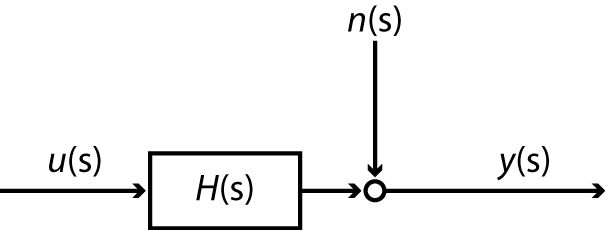
\includegraphics{images/SISOblock}
		%		\caption{Blockdiagram of the SISO model}
		\label{fig:SISOblock}
	\end{center}
	Where $u = u(s)$ represents the steering torque $T_\delta$ input, $\hat{y}= y(s)$ represents the measured output and $n= n(s)$ represents the measurement noise. 
\subsection{Simulation}
The linearized benchmark equations are used for the simulation. A forward velocity of 5 m/s is chosen, which results in stable dynamic behavior of the bicycle. The transferfunction from steering torque $T_\delta$ to roll angle $\phi$ is derived and yields (in zero-pole-gain form):
\begin{align}
H =   \frac{  -0.12262 (s+58.91) (s+13.77)  }{ (s+0.35) (s+14.27) (s^2 + 1.594s + 19.53) } 
\end{align}
This model will be used to simulate the bicycle response. Later on we will assume the system to be unknown and use system identification and parameter estimation techniques to estimate the  transfer function. Naturally the following question arises; ''why bother estimating a system that is already known?'. De answer to this this question is that we are actually interested in the quality of the identification procedures. The quality of the estimated fit can easily be checked by comparing it with the true system.

A simulation is set up, using the following measurement parameters:
			\begin{center}
				\begin{tabular}{lccc}
				\toprule
				description & symbol & value & units  \\
				\midrule
					Measurement time	 &	T    					& $100	$							& [s] 		\\
					Sample frequency	 &		$f_s$   			& $50		$							& [Hz] 	\\
					Sample period				 &	$\Delta T$ & $1/f_s$ 							& [s] 		\\
					Number of samples &		$N$    			& $T/\Delta T	$			& [-]			\\
					Input bandwidth & $f_{bw}$ & $2$                   & [Hz] \\
					\bottomrule
				\end{tabular}
			\end{center}
The input signal $u$ is designed as an crested multisine, which is described in the previous chapter. The maximum torque is set to 0.6 Nm. The standard deviation of the noise is set to 0.01 rad.
Next the simulation is started resulting in the measured output $y(t)$. The input and output are then converted to the frequency domain, spectral densities are calculated and finally some frequency averaging (not discussed) is applied in order to reduce the noise.
\subsection{System identification}
Next we will use the simulated dataset to derive the transfer function of the system. Starting from the block diagram shown in figure \ref{fig:SISOblock} we can derive the following equation:
\begin{align}
		Hu & = y-n 
\end{align}
Unfortuneatly we don't know the the noise $n$, which makes solving for $H$ impossible. However we can find a linear estimation of the system by seeking a solution under the image of $u$. This is achieved by projecting $u$ onto the left side of the equations. Assuming the noise is uncorrelated with the input (they are 2  independent signals), the linear estimated transferfunction $\hat{H}$ can be derived:
\begin{align}
		u^\ast Hu & = u^\ast (y-n) \nonumber \\
		H 					& = \frac{u^\ast (y-n)}{u^\ast u}  \nonumber \\
		\hat{H}	& = \frac{u^\ast y}{u^\ast u} \nonumber \\
		\hat{H} 	& = \frac{S_{uy}}{S_{uu}}
		\label{eq:SISOH}
\end{align}
Here $S_{uy}$ represent the cross spectral density of the input/output and $S_{uu}$ represents the auto spectral density of the input. The resulting tranferfunction is shown as a bode function in figure \ref{fig:SISObode}. The gain of the transfer function decreases as the frequency increases, resulting in a poorer signal to noise ratio at higher frequencies. Also notice that the input signal contains frequency content ranging from 0 to 2 Hz. Above 2 Hz the response is dominated completly by the noise. The coherence represents the linear estimation quality of the transfer function. As expected, the coherence drops dramatically above 2 Hz.
	\begin{figure}
		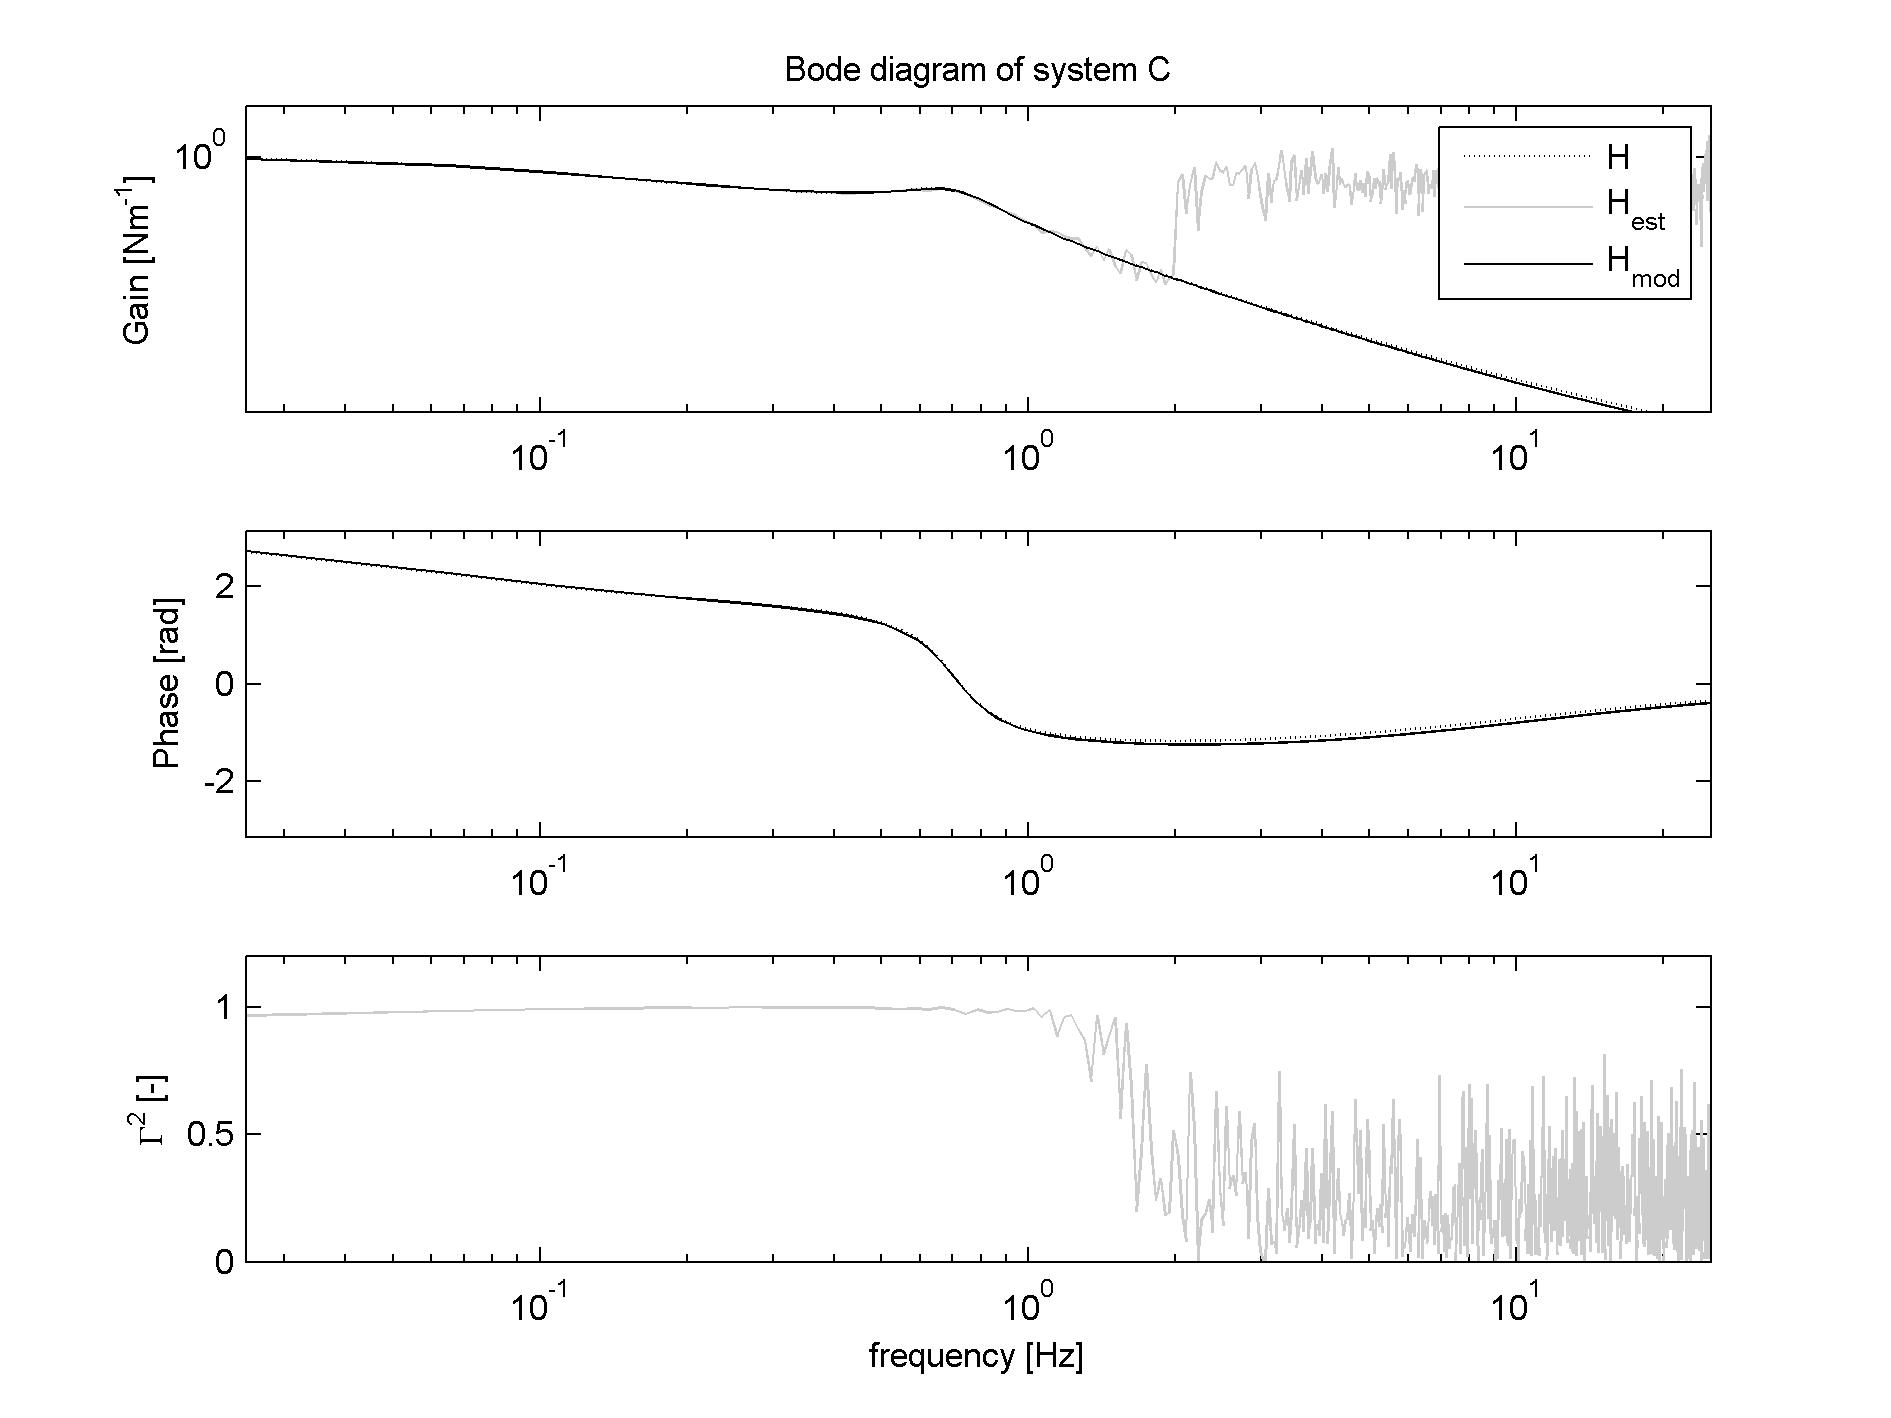
\includegraphics{images/SISObode}
		\caption{Bode diagram of the true ($H$), estimated ($H_{est}$) and parametric ($H_{mod}$) transfer function.}
				\label{fig:SISObode}
	\end{figure}
\subsection{Parameter estimation}
The estimated tranferfunction can then be used to determining the actual parameters of the transferfunction. We assume a solution of the following form:
	\begin{align}
		H_{\textrm{mod}}(s,x_i) = \frac{ x_1 (s+x_2) (s+x_3)  }{ (s+x_4) (s+x_5) (s^2 + x_6s + x_7) } 
	\end{align}
The error function is chosen to be:
		\begin{equation}
		e_s = \sqrt{\frac{1}{2\pi\omega_s}}\gamma(\omega_s)\left|\ln \hat{H}(\omega_s)-\ln H_{mod}(\omega_s,x_i)\right|
		\end{equation}
Here the $1\omega$ term acts as a weightening function, which puts more weight on lower frequencies. The $\ln$ function puts more weight on errors at lower magnitudes. This error definition is commonly used when fitting in the frequency domain. The reason to use these special weightnings is to counteract the logarithmic scale of a bode magnitude plot.
The criterium thus becomes:
		\begin{equation}
		J = \frac{1}{2}\sum_{s} e_s^2
		\end{equation}	
The Matlab \mcode{lsqnonlin} algorithm is used for the optimization. The resulting parameters together with the true parameters are shown in table \ref{table:SISOparms}.
\begin{table}
\centering
		\begin{tabular}{cccc}
		\toprule
		$x_i$ & True & Estimated & $\sigma_{\mu_{x_i}}$ \\
		\midrule
		$x_1$&   -0.1112  	& -0.1226  	&  0.1241\\
		$x_2$&	58.0972   	&58.9100  	& 89.8280\\
    $x_3$&	7.3382   		&13.7700  	& 35.0404\\
    $x_4$&	0.3715   		& 0.3500  		&  0.0295\\
    $x_5$&	6.6603   		&14.2700  	& 29.0601\\
    $x_6$&	1.5845    	&1.5940  		&  0.1576\\
		$x_7$&	19.7927  	&19.5300 		&   0.6974\\
		\bottomrule
 		\end{tabular}
		\caption{Comparison of the estimated parameters with the true parameters. $\sigma_{\mu_{x_i}}$ represents the standard deviation of the mean.}
		\label{table:SISOparms}
\end{table}
The quality of the resulting parameters is varying. Some parameters ar more difficult to fit than others. When we look at the true system (equation \ref{eq:SISOH}), we observe a near zero/pole cancelation of the 3th and 5th parameter, which renders them practically unobservable. This makes these parameters very hard to  fit, which results in a huge uncertainty in the estimation these 2 corresponding parameters. The low quality fit of parameter 2 is unknown at this point. Possibly the optimization algorithm got stuck on a global minimum. The resulting fit (shown in figure \ref{fig:SISObode} seems pretty good however.